%%%%%%%%%%%%%%%%%%%%%%%%%%%%%%%%%%%%%%%%%%%%%%%%%%%%
%%%%%%%%%%%%%%%%%%%%%%%%%%%%%%%%%%%%%%%%%%%%%%%%%%%%%%%%%%%%%%%%%%%%%%
% Chapitre 5
\chapter{Chapitre 5 : Réalisation}

%%%%% Intro Chapitre 4
\section*{Introduction}
\phantomsection
\addcontentsline{toc}{section}{Introduction}

\paragraph{}\begin{spacing}{2}
Dans ce chapitre, nous allons survoler les différents choix techniques pour lesquels nous avons opté, et présenter l’application dans sa globalité.
\end{spacing}
\vspace{4cm} 

\newpage
\section{Méthodologie de développement}
\subsection{Langage UML}
\paragraph{}
De nos jours, pour pouvoir spécifier et exprimer les besoins et les exigences des acteurs, du système et de l’architecture globale, plusieurs outils de modélisation de processus métier se sont présentés.

\includegraphics[width=\linewidth, height=5cm]{images/UML_logo.svg.png}

\paragraph{}
La modélisation \textbf{UML} permet de vulgariser les aspects liés à la conception et à l’architecture, propres au logiciel, au client. Aussi, elle apporte une compréhension rapide du programme à d’autres développeurs externes en cas de reprise du logiciel et facilite sa maintenance.
\paragraph{}
L’utilisation d’UML varie en fonction du type d’application à réaliser, et de sa taille. Par exemple, sur les douze diagrammes que contient UML, deux ou trois suffisent à réaliser un petit projet. Il faut savoir qu’un modèle doit avoir un objectif précis. Sinon, il risque de ne pas être adapté à son usage.

\textbf{Exemples de diagrammes} :
\begin{itemize}
    \item Le diagramme de cas d’utilisation,
    \item Les diagrammes de séquence,
    \item Le diagramme d'activité.
\end{itemize}
\subsubsection*{Justification du choix d’UML}
\paragraph{}
UML est avant tout un support de communication performant, qui facilite la représentation et la compréhension de solutions orientées objet.
\paragraph{}
L'aspect formel de sa notation limite les ambiguïtés et les incompréhensions. Son indépendance par rapport aux langages de programmation, aux domaines d'application et aux processus, en fait un langage universel.
\paragraph{}
UML, contrairement à son prédécesseur \textbf{MERISE} qui est une méthode systémique (orientée données), donne un sens intéressant à l'approche objet et couvre de plus tout le cycle de réalisation du logiciel.

\subsection{CrewAI }
\paragraph{}
CrewAI est une plateforme qui permet aux développeurs de construire et de déployer des flux de travail automatisés en utilisant plusieurs agents d'intelligence artificielle qui collaborent pour effectuer des tâches complexes.

\paragraph{}
Les agents d'IA sont des assistants capables d'effectuer des tâches et d'interagir avec le monde. Contrairement aux systèmes traditionnels qui suivent des règles fixes, ils peuvent apprendre et s'adapter à de nouvelles situations. Considérez-les comme des robots intelligents qui vous aident à accomplir toute une série de tâches.
\paragraph{}
Mais qu'est-ce qui différencie les agents d'intelligence artificielle des autres entités d'intelligence artificielle, comme les populaires modèles de langage dont nous avons tous entendu parler ?
\paragraph{}
Dans cet article, je vais répondre à cette question et vous présenter CrewAI, un framework Python gratuit et open-source conçu pour simplifier le développement de systèmes d'IA multi-agents. Nous étudierons la distinction entre les agents et les modèles de langage, nous discuterons des raisons pour lesquelles les cadres d'agents sont importants pour la construction d'applications d'IA. construire des applications d'IAet nous montrerons comment CrewAI permet aux agents de collaborer et d'obtenir d'excellents résultats.
\subsubsection{Agents d'IA vs. LLMs }
\paragraph{}
Démystifions un malentendu courant concernant la différence entre les agents et les grands modèles linguistiques (LLM). Tous deux appartiennent à la famille de l'intelligence artificielle, mais ils possèdent des capacités distinctes.

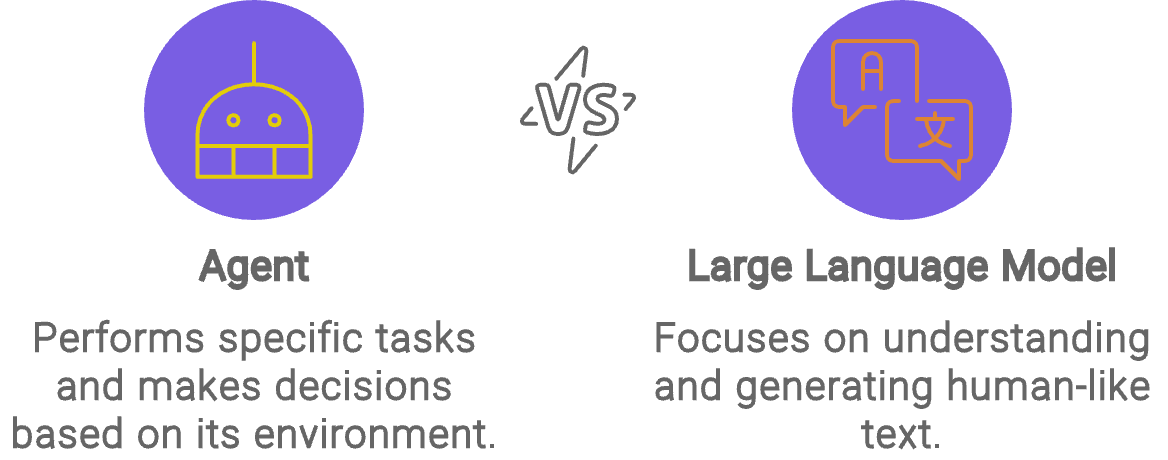
\includegraphics[width=\linewidth, height=5cm]{images/agentVsLLM.png}

\paragraph{}
Les modèles linguistiques, tels que ChatGPT et Geminisont très habiles dans l'utilisation du langage. Ils ont suivi une formation approfondie sur de grandes quantités de textes et de codes, ce qui les a dotés de la capacité de comprendre et de produire un langage qui ressemble beaucoup à la communication humaine.

\paragraph{}
Les LLM sont d'habiles faiseurs de mots de l'intelligence artificielle, produisant un large éventail de contenus, y compris des traductions, des résumés, des récits créatifs ou même de la poésie. Leur champ d'application est généralement limité auxtâches liées à la langue .

\paragraph{}
Les agents, quant à eux, se concentrent principalement sur l'action. Ils sont capables de naviguer, d'interagir avec des objets et de prendre des décisions sur la base de leurs perceptions. 

\paragraph{}
En bref, les modèles linguistiques sont des cerveaux et les agents sont des mains. Ensemble, ils forment un duo puissant.

\paragraph{}
Les agents jouant un rôle essentiel dans les applications d'IA, comment gérer leur complexité lorsque plusieurs agents doivent travailler ensemble ? C'est là qu'interviennent les cadres d'agents.

\subsubsection{La nécessité d'un cadre pour les agents }

\paragraph{}
Le besoin de cadres d'agents découle de la complexité croissante des applications de l'IA, en particulier celles qui impliquent plusieurs agents travaillant en collaboration pour atteindre un objectif commun. Voyons pourquoi les cadres d'agents sont essentiels.   

\subsubsection{Orchestration et coordination }

\paragraph{}
À mesure que les systèmes d'IA prennent de l'ampleur, ils intègrent souvent de nombreux agents dotés de capacités diverses. Il devient de plus en plus difficile de gérer ces interactions et de s'assurer qu'elles fonctionnent harmonieusement.

\paragraph{}
Les cadres d'agents offrent un environnement structuré qui permet d'orchestrer les activités des agents, de définir leurs rôles et responsabilités et d'améliorer la communication.
\paragraph{}
Dans les systèmes multi-agents, un aspect important est l'attribution efficace des tâches aux agents les plus appropriés et la gestion efficace des ressources partagées. Les cadres d'agents fournissent des mécanismes dynamiques pour la répartition des tâches, la négociation des ressources et la résolution des conflits.

\subsubsection{Qu'est-ce que CrewAI ? }
\paragraph{}
CrewAI est un framework Python open-source conçu pour soutenir le développement et la gestion de systèmes d'IA multi-agents.
\paragraph{}
CrewAI améliore ces systèmes d'IA en attribuant des rôles spécifiques, en permettant une prise de décision autonome et en facilitant la communication entre les agents. Cette approche leur permet de s'attaquer à des problèmes complexes plus efficacement que des agents travaillant seuls.


\includegraphics[width=\linewidth, height=5cm]{images/crewai.png}
 
\noindent
Ce cadre se compose d'une série d'outils, notamment des moteurs de recherche sur le web et des modèles linguistiques, qui permettent aux agents d'entrer en contact avec le monde extérieur, de collecter des informations et d'agir pour atteindre leurs objectifs.

\medskip

\noindent
La conception et l'évolutivité de CrewAI en font un outil idéal pour le développement d'applications multi-agents simples et complexes, encourageant une méthode collaborative pour relever les défis et prendre des décisions au sein des systèmes d'IA.

\medskip

\noindent
Examinons quelques-unes des principales caractéristiques qui font de CrewAI un outil puissant pour la construction de systèmes multi-agents.

\paragraph{\textbf{Orchestration d'agents :}} CrewAI veille à ce que chaque agent connaisse son rôle dans la performance. Il fournit les outils nécessaires pour définir et coordonner les comportements des agents, afin de s'assurer que tout le monde joue en synchronisation.

\paragraph{\textbf{Architecture basée sur les rôles :}} Comme pour l'attribution de différents instruments aux musiciens, CrewAI vous permet d'attribuer des rôles spécifiques aux agents, en définissant leurs capacités et leurs autorisations. Cela permet de créer un système modulaire et bien structuré, même lorsque les choses deviennent complexes.

\paragraph{\textbf{Une communication souple :}} CrewAI prend en charge différents canaux de communication, ce qui permet aux agents d'échanger des informations en toute transparence. Pensez-y comme si vous disposiez d'un chat privé, d'une discussion de groupe et d'un mégaphone en un seul et même endroit.

\paragraph{\textbf{Intégration des outils :}} CrewAI permet aux agents d'interagir avec le monde grâce à différents outils. Ces outils permettent aux agents d'effectuer des recherches sur le web, de comprendre le langage, d'analyser des données et d'effectuer des tâches personnalisées.

\paragraph{\textbf{Évolutivité :}} CrewAI est conçu pour s'adapter sans effort, garantissant que votre système multi-agents reste réactif et efficace au fur et à mesure de sa croissance.

\medskip

\noindent
Mais quels sont les avantages que CrewAI apporte au tableau ? Voyons quels sont ses avantages.

\subsection*{Avantages de l'utilisation de CrewAI}

\noindent
Crew.ai permet à plusieurs agents d'intelligence artificielle de collaborer, de partager leurs connaissances et de coordonner leurs actions en vue d'atteindre un objectif commun.

\medskip

\noindent
En automatisant la distribution des tâches et la gestion des ressources, Crew.ai permet aux agents de se concentrer sur leurs rôles spécifiques avec un minimum de frais généraux.

\medskip

\noindent
Le cadre prend également en charge l'adaptabilité, ce qui permet aux agents d'ajuster leur comportement en fonction de l'évolution des conditions ou des objectifs.

\medskip

\noindent
En outre, Crew.ai simplifie le processus de développement grâce à une plateforme conviviale pour la création et la gestion de systèmes multi-agents.
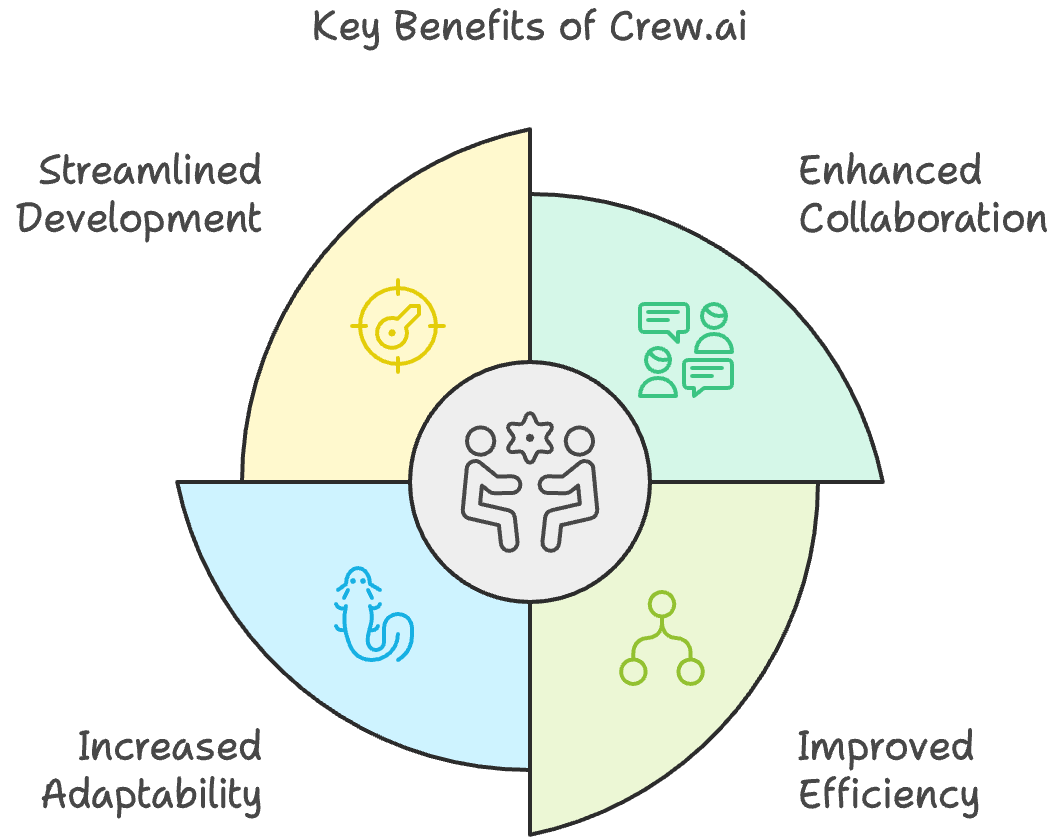
\includegraphics[width=\linewidth, height=7cm]{images/key benefits of.png}

\paragraph{}
Un autre point fort de CrewAI est son intégration avec une large gamme d'outils. Cela étend les capacités des agents, leur permettant d'interagir avec le monde extérieur et de recueillir des informations.
\paragraph{}
CrewAI prend en charge des outils tels que des moteurs de recherche web, des modèles de langage, des outils d'analyse de données et même des fonctionnalités personnalisées. Cela permet aux agents d'effectuer des tâches qui dépassent leurs capacités de base, telles que la recherche d'informations sur le web ou l'analyse de données complexes.

\subsection{Ollama  }

\paragraph{}
Ollama est un outil open-source qui exécute de grands modèles de langage (LLM) directement sur une machine locale . Il est donc particulièrement intéressant pour les développeurs d’IA, les chercheurs et les entreprises soucieuses du contrôle des données et de la protection de la vie privée.
\paragraph{}
En exécutant les modèles localement, vous conservez l’entière propriété des données et évitez les risques de sécurité potentiels associés au stockage dans le cloud. Les outils d’IA hors ligne comme Ollama contribuent également à réduire la latence et la dépendance à l’égard des serveurs externes, ce qui les rend plus rapides et plus fiables.
\paragraph{}
Cet article explore les principales caractéristiques d’Ollama, les modèles pris en charge et les cas d’utilisation pratiques. À la fin, vous serez en mesure de déterminer si cet outil LLM convient à vos projets et à vos besoins en matière d’IA.

\section*{Comment fonctionne Ollama}

Ollama crée un environnement isolé pour exécuter les LLM localement sur votre système, ce qui évite tout conflit potentiel avec d’autres logiciels installés. Cet environnement comprend déjà tous les composants nécessaires au déploiement de modèles d’IA, tels que :

\begin{itemize}
    \item \textbf{Poids du modèle.} Les données pré-entraînées que le modèle utilise pour fonctionner.
    \item \textbf{Fichiers de configuration.} Paramètres qui définissent le comportement du modèle.
    \item \textbf{Dépendances nécessaires.} Bibliothèques et outils qui soutiennent l’exécution du modèle.
\end{itemize}

\noindent
Pour simplifier, vous tirez d’abord des modèles de la bibliothèque d’Ollama. Ensuite, vous exécutez ces modèles tels quels ou vous ajustez les paramètres pour les adapter à des tâches spécifiques. Après la configuration, vous pouvez interagir avec les modèles en entrant des invites, et ils génèrent les réponses.

\medskip

\noindent
Cet outil d’IA avancé fonctionne mieux sur les systèmes à unité de traitement graphique (GPU) dédiée. Bien que vous puissiez l’exécuter sur des GPU intégrés au CPU, l’utilisation de GPU compatibles dédiés, comme ceux de NVIDIA ou d’AMD, réduira les temps de traitement et garantira des interactions plus fluides avec l’IA.

\medskip

\noindent
Nous recommandons de consulter la page GitHub officielle d’Ollama pour vérifier la compatibilité avec les GPU.

\section*{Principales caractéristiques d’Ollama}

Ollama offre plusieurs fonctionnalités clés qui facilitent la gestion des modèles hors ligne et améliorent les performances.

\subsection*{Gestion locale des modèles IA}

Ollama vous permet de télécharger, de mettre à jour et de supprimer facilement des modèles sur votre système. Cette fonctionnalité est précieuse pour les développeurs et les chercheurs qui accordent une grande importance à la sécurité des données.

\medskip

Outre la gestion de base, Ollama vous permet de suivre et de contrôler les différentes versions du modèle. Cette fonction est essentielle dans les environnements de recherche et de production, où il peut être nécessaire de revenir à plusieurs versions de modèles ou de les tester pour déterminer celle qui produit les résultats souhaités.

\subsection*{Options de la ligne de commande et de l’interface graphique}

Ollama fonctionne principalement via une interface de ligne de commande (CLI), ce qui vous donne un contrôle précis sur les modèles. L’interface de ligne de commande permet des commandes rapides pour extraire, exécuter et gérer les modèles, ce qui est idéal si vous êtes à l’aise pour travailler dans une fenêtre de terminal.

\medskip

Si vous êtes intéressé par une approche en ligne de commande, n’hésitez pas à consulter notre tutoriel Ollama CLI.

\medskip

Ollama prend également en charge des outils d’interface utilisateur graphique (GUI) tiers, tels que Open WebUI, pour ceux qui préfèrent une approche plus visuelle.

\section{Quoi de neuf avec LLaMA 3.2 ?}
\begin{itemize}
    \item LLaMA 3.2 est une mise à jour importante qui améliore la version 3.
    \item Optimisations dans l’architecture et les algorithmes d’entraînement permettant :
    \begin{itemize}
        \item Une meilleure compréhension contextuelle.
        \item Une génération de texte plus naturelle et précise.
        \item Une meilleure gestion des longues séquences textuelles.
    \end{itemize}
    \item Amélioration des performances sur des benchmarks standards de traitement automatique du langage naturel (NLP).
    \item Support amélioré pour plusieurs langues avec une meilleure compréhension multilingue.
\end{itemize}

\subsection{Architecture technique}
\begin{itemize}
    \item Basé sur l’architecture \textbf{Transformer}, norme dans les modèles de langage modernes.
    \item Plusieurs tailles de modèles disponibles, allant de quelques milliards à plusieurs dizaines de milliards de paramètres.
    \item Techniques avancées d’entraînement :
    \begin{itemize}
        \item Apprentissage auto-supervisé sur de vastes corpus textuels.
        \item Algorithmes d’optimisation modernes accélérant la convergence.
    \end{itemize}
    \item Utilisation de régularisation pour éviter le surapprentissage et améliorer la généralisation.
\end{itemize}

\subsection{Performances et benchmarks}
\begin{itemize}
    \item LLaMA 3.2 se positionne parmi les meilleurs modèles open source ou semi-open source.
    \item Rapprochement des performances avec des modèles commerciaux comme GPT-4 ou PaLM sur plusieurs tâches :
    \begin{itemize}
        \item Réponse aux questions.
        \item Traduction.
        \item Résumé automatique.
        \item Raisonnement logique.
    \end{itemize}
    \item Bon équilibre entre taille du modèle, coût de calcul et performance.
\end{itemize}

\subsection{Points forts de LLaMA 3.2}
\begin{itemize}
    \item \textbf{Efficacité} : Moins gourmand en ressources matérielles (GPU/TPU) comparé à certains concurrents.
    \item \textbf{Modularité} : Plusieurs tailles disponibles, permettant un déploiement flexible (serveurs, cloud, local).
    \item \textbf{Accessibilité} : Partiellement open source ou accessible sous licence, favorisant la recherche.
    \item \textbf{Robustesse linguistique} : Meilleure compréhension des nuances, contextes longs et langues multiples.
    \item \textbf{Adaptabilité} : Facilité de fine-tuning pour des domaines spécifiques (santé, finance, droit...).
\end{itemize}

\subsection{Cas d’usage concrets}
\begin{itemize}
    \item Assistants virtuels intelligents (service client, support technique).
    \item Création de contenu (rédaction, génération créative).
    \item Traduction multilingue pour plateformes internationales.
    \item Analyse de sentiments et modération de contenu.
    \item Synthèse et résumé automatique de documents.
    \item Recherche et extraction d’informations dans des bases textuelles.
\end{itemize}

\subsection{Enjeux et limites}
\begin{itemize}
    \item \textbf{Éthique et biais} : Le modèle peut refléter des biais présents dans les données d’entraînement.
    \item \textbf{Sécurité} : Risques d’usage malveillant (désinformation, deepfakes textuels).
    \item \textbf{Complexité du déploiement} : Nécessite des ressources matérielles importantes pour les grands modèles.
    \item \textbf{Dépendance aux données} : La qualité des données impacte directement la performance.
\end{itemize}

\subsection{Perspectives futures}
\begin{itemize}
    \item Améliorations continues via :
    \begin{itemize}
        \item Meilleurs algorithmes d’apprentissage.
        \item Données d’entraînement plus diverses et de meilleure qualité.
        \item Intégration avec d’autres technologies d’IA (vision, audio).
    \end{itemize}
    \item Déploiements élargis dans des applications industrielles et grand public.
    \item Outils facilitant la personnalisation et l’interaction utilisateur.
\end{itemize}

\subsection{Streamlit}
\paragraph{}
Streamlit est un framework gratuit et open-source qui permet de créer et de partager rapidement de superbes applications web d'apprentissage automatique et de science des données.
\paragraph{}
Il s'agit d'une bibliothèque basée sur Python spécifiquement conçue pour les ingénieurs en apprentissage automatique. Les scientifiques des données ou les ingénieurs en apprentissage automatique ne sont pas des développeurs web et ils n'ont pas envie de passer des semaines à apprendre à utiliser ces frameworks pour créer des applications web. Ils souhaitent plutôt un outil plus facile à apprendre et à utiliser, pour autant qu'il puisse afficher des données et collecter les paramètres nécessaires à la modélisation.
\paragraph{}
Streamlit vous permet de créer une application à l'apparence étonnante avec seulement quelques lignes de code.
 
\includegraphics[width=\linewidth, height=7cm]{images/streamlit-logo-secondary-colormark-darktext.png}

 \paragraph{}
 L'avantage de Streamlit est que vous n'avez même pas besoin de connaître les bases du développement web pour commencer ou pour créer votre première application web. Si vous êtes un adepte de la science des données et que vous souhaitez déployer vos modèles facilement, rapidement et avec seulement quelques lignes de code, Streamlit est un bon choix.

 \paragraph{}
L'un des aspects importants de la réussite d'une application consiste à la doter d'une interface utilisateur efficace et intuitive. La plupart des applications modernes, gourmandes en données, sont confrontées au défi de créer rapidement une interface utilisateur efficace, sans passer par des étapes compliquées. Streamlit est une bibliothèque Python open-source prometteuse, qui permet aux développeurs de créer des interfaces utilisateur attrayantes en un rien de temps.

\paragraph{}
Streamlit est le moyen le plus simple, en particulier pour les personnes qui n'ont pas de connaissances en matière d'interface, d'intégrer leur code dans une application web :

\begin{itemize}
    \item Aucune expérience ou connaissance en matière d'interface (html, js, css) n'est requise.
    \item Vous n'avez pas besoin de passer des jours ou des mois à créer une application web, vous pouvez créer une très belle application d'apprentissage automatique ou de science des données en seulement quelques heures ou même quelques minutes.
    \item Il est compatible avec la majorité des bibliothèques Python (par exemple pandas, matplotlib, seaborn, plotly, Keras, PyTorch, SymPy (latex)).
    \item Moins de code est nécessaire pour créer des applications web étonnantes.
    \item La mise en cache des données simplifie et accélère les pipelines de calcul.
\end{itemize}

\section{Base de Données : MySQL}
\paragraph{}
MySQL est un système de gestion de base de données relationnelle open source. Il est utilisé pour stocker et gérer les données collectées par les capteurs, les informations des utilisateurs et les historiques des données. MySQL est connu pour sa performance, sa fiabilité et sa facilité d'utilisation.

 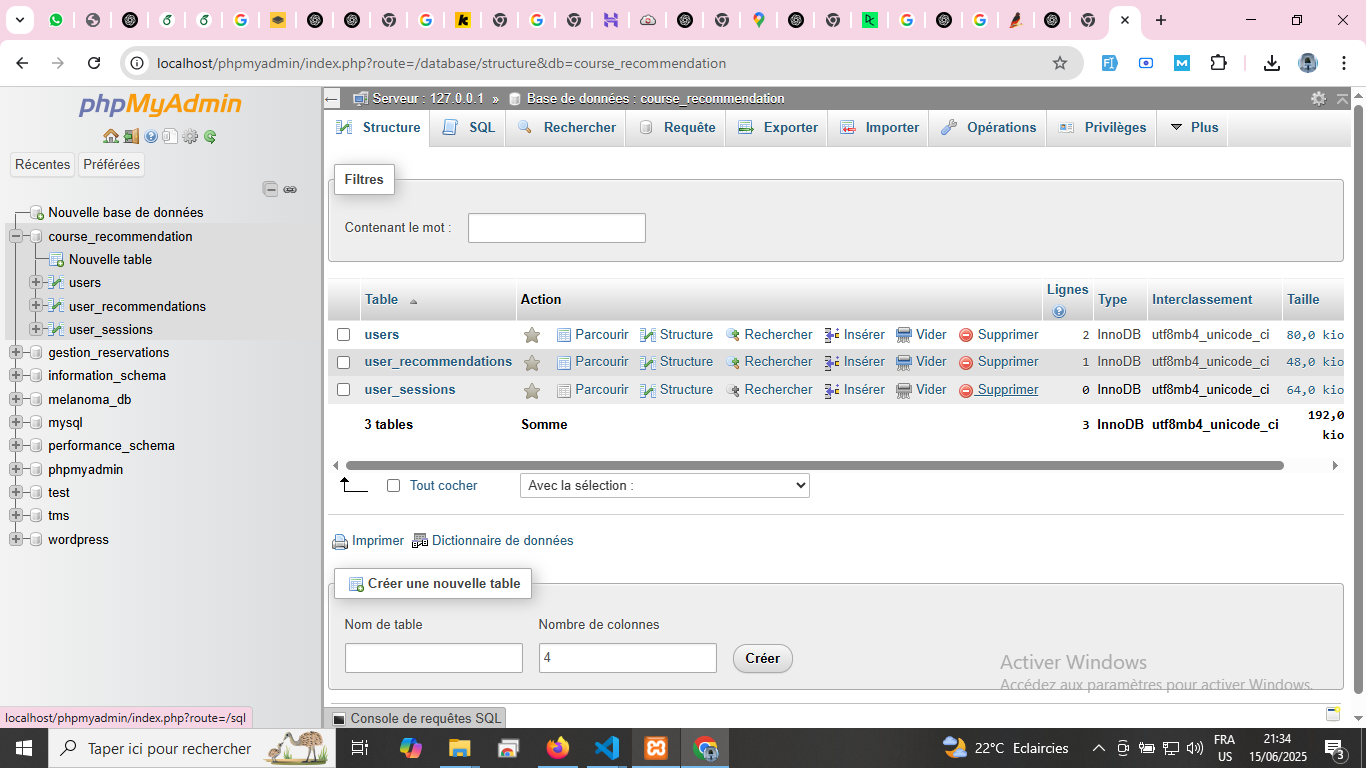
\includegraphics[width=\linewidth, height=7cm]{images/Capture d’écran (200).png}
\newpage
 \section{Procédure de Déploiement de l'Application Streamlit}

Cette section décrit les étapes nécessaires pour déployer l'application développée avec le framework \textbf{Streamlit}.

\subsection{1. Pré-requis}

Avant de procéder au déploiement, assurez-vous que les éléments suivants sont installés sur la machine :

\begin{itemize}
  \item Python 3.8 ou version supérieure
  \item pip (gestionnaire de paquets Python)
  \item Git (facultatif si vous clonez un dépôt)
  \item Un environnement virtuel (recommandé)
\end{itemize}

\subsection{2. Création et activation de l'environnement virtuel}

\begin{verbatim}
python -m venv env
source env/bin/activate        % Sous Linux ou macOS
env\Scripts\activate           % Sous Windows
\end{verbatim}

\subsection{3. Installation des dépendances}

Installez les bibliothèques nécessaires à partir du fichier \texttt{requirements.txt} :

\begin{verbatim}
pip install -r requirements.txt
\end{verbatim}

\subsection{4. Lancement de l'application en local}

Utilisez la commande suivante pour démarrer l’application Streamlit en local :

\begin{verbatim}
streamlit run app.py
\end{verbatim}

où \texttt{app.py} est le fichier principal de votre application.

\subsection{5. Déploiement sur une plateforme en ligne (facultatif)}

Il est possible de déployer l'application sur des plateformes telles que :

\begin{itemize}
  \item \textbf{Streamlit Cloud} (\url{https://streamlit.io/cloud})
  \item \textbf{Render} (\url{https://render.com})
  \item \textbf{Heroku} (\url{https://www.heroku.com})
\end{itemize}

\subsubsection*{Exemple de déploiement sur Streamlit Cloud :}

\begin{enumerate}
  \item Créer un dépôt sur GitHub et y pousser votre code.
  \item Aller sur \url{https://streamlit.io/cloud} et se connecter.
  \item Cliquer sur \texttt{New app}, sélectionner le dépôt GitHub.
  \item Indiquer le nom du fichier principal (\texttt{app.py}).
  \item Lancer le déploiement.
\end{enumerate}

\subsection{6. Mise à jour de l'application}

Pour mettre à jour l’application en ligne :

\begin{itemize}
  \item Effectuer les modifications localement.
  \item Pousser les changements sur GitHub.
  \item La plateforme de déploiement redémarre automatiquement l’application avec les nouvelles modifications.
\end{itemize}

\subsection{7. Résolution des problèmes}

Quelques commandes utiles pour déboguer :

\begin{itemize}
  \item \texttt{streamlit logs} : pour consulter les journaux
  \item \texttt{pip list} : pour vérifier les packages installés
\end{itemize}

